% Online Appendix to Section 4 (sec:normalization). Specification: R/utils/scurve.R,
% R/indices/index_builder_core.R, config/index_definition.yml, config/missing_data.yml,
% config/weights.yml, config/rankability.yml. Numbers: paper/results/method.json and scurve.json
% (final rerun of 12 October 2026).
\section{Index construction: derivations and further diagnostics}\label{oa:normalization}

This appendix collects the construction algorithm, the properties of the S-curve that Section~\ref{sec:normalization}
uses without proof, the conventions of the theme and aggregation layers, and the diagnostics of
the final build that the main text summarises.

\begin{algorithm}[t]
  \caption{Construction of a pillar index $P\in\{\ES,\EO\}$ from its theme tables}
  \label{alg:pillar}
  \begin{algorithmic}[1]
    \Require theme tables $h\in\mathcal H_P$; category weights $w_k$
      (\texttt{config/weights.yml}); missing-data rules $m_h\in\{\text{zero},
      \text{global average}\}$ (\texttt{config/missing\_data.yml}); for each category its
      score variable and components $\mathcal V_{k}$ (\texttt{config/index\_definition.yml})
    \State Bind the theme tables; average rows that differ only by sub-sector; keep rows whose
      data type is \emph{index}
    \State For each $(i,t,s,k,v,h)$ keep the observation with the latest year
      \Comment{eq.~\eqref{eq:latest_year}}
    \For{each technology--stage pair $(t,s)$}
      \State Complete the grid of economies $\times$ component groups
      \For{each group $g=(t,s,k,v,h)$}
        \If{at least one economy is observed in $g$ and theme $h$ has a rule}
          \State Fill the missing economies of $g$ by rule $m_h$ from the observed values
          \Comment{eq.~\eqref{eq:impute}}
        \EndIf
      \EndFor
    \EndFor
    \State Average each component over themes; score each category by the mean of its present
      components \Comment{eq.~\eqref{eq:overall}}
    \State Aggregate the observed categories of each cell with renormalised weights
      \Comment{eq.~\eqref{eq:pillar}}
    \State Record category and variable contributions, $\iota_{its}$ and the pair status; flag
      rankable cells \Comment{eqs.~\eqref{eq:cat_decomp}--\eqref{eq:rankable}}
    \Ensure $P_{its}\in[0,1]$, or missing when no category of the cell is observed
  \end{algorithmic}
\end{algorithm}

\paragraph{Theme tables and orientation.} Every theme table has one row per economy, technology,
stage, sub-sector, category, variable, data type and year, with its value, source and a short
explanation. Rows of type \emph{raw} keep a metric in natural units for tracing; only rows of type
\emph{index}, on $[0,1]$, enter the pillars. Rows that differ only by sub-sector are averaged with
equal weights before any other step. Each variable is oriented in its theme: concentration enters
through $-\HHI$, a trade deficit relative to GDP, a levelised cost and price volatility through
their negatives. By the symmetry of $\Scurve$, the S-curve of $-x$ is one minus the S-curve of $x$
for any comparison set with at least two observations, so orientation and transformation commute.
The opportunity builder verifies that every category score lies in $[0,1]$.

\paragraph{The S-curve.} Differentiating equation~\eqref{eq:scurve},
\begin{equation}\label{eq:scurve_slope}
  \Scurve'(r)=\frac{\gamma\,[r(1-r)]^{\gamma-1}}{\bigl[r^{\gamma}+(1-r)^{\gamma}\bigr]^{2}},
  \qquad \Scurve'(1/2)=\gamma ,
\end{equation}
which for $\gamma<1$ diverges as $r\to0$ or $r\to1$. With $\gamma=0.5$ the quartiles map to
0.366 and 0.634, so near the median a step in rank moves the index by half as much as it moves the
percent rank, while gaps between adjacent units are widened in the tails. In levels, $\Scurve(r)>r$
below the median and $\Scurve(r)<r$ above it. With $n$ untied observations the index takes exactly
the values $\Scurve(k/(n-1))$, $k=0,\dots,n-1$, whatever the raw distribution, so every untied
S-curved variable has mean $1/2$ and a dispersion that depends only on $n$ and $\gamma$: the
population standard deviation is 0.260 for $n=10$, 0.224 for $n=20$ and 0.206 for $n=40$, and
tends to 0.19, against 0.29 for the percent rank and 0.38 for $\gamma=2$. Components ranked over
comparison sets of a given size therefore enter a category on a common scale; smaller sets have
larger spreads, and ties, the zero anchor and imputed values move a component away from the grid.
The smallest step above zero, $\Scurve(1/(n-1))$, is coarse in small sets (0.261 for $n=10$,
0.140 for $n=40$). A single observation scores 0, two score 0 and 1, and a fully tied set scores
$1/2$. In the simulated lognormal sample of Figure~\ref{fig:scurve}, min-max rescaling puts 29 of
40 observations below 0.1 and spreads the top four over 0.79 of the scale; the percent rank gives
each group of four a spread of 0.077; the S-curve gives the bottom and top four 0.22 each and the
middle four 0.04. Rank-based normalisation is a standard option for composite indicators
\citep{oecd2008handbook}; it is adopted because the inputs differ in units and skewness by orders
of magnitude and the questions the indices answer are comparative. Min-max or $z$-score
normalisation would let a few very large values compress the rest of the distribution.

\paragraph{The zero anchor.} Equation~\eqref{eq:scurve_zero} is equation~\eqref{eq:scurve}
applied to the positive values with a single zero prepended to the comparison set and then
removed. An observed zero and an unrecorded economy both score 0, and the smallest positive value
scores $\Scurve(1/m)>0$: for $(0,2,5,9)$ the positive entries score 0.414, 0.586 and 1. A set in
which every value is zero scores 0 throughout.

\paragraph{Comparison sets and cardinal exceptions.} Most themes rank the economies observed in a
pair, sometimes split by sub-sector, year or mineral before averaging to the pair. World-level
series are ranked across the units over which they vary: commodity-price volatility across
technologies, world export concentration across the cells of the eleven headline technologies, and
global demand across fuels. A theme that builds a composite of several S-curved terms averages
them and may pass the average through the S-curve again. Index values are positions in a
cross-section: adding or removing economies changes the scores of the others, and a change over
time records a change in standing against the field. The three cardinal $\EO$ inputs are the
readiness score (a raised-cosine bell in the readiness level, zero at levels 2 and 11 and peaking
at 6, blended 0.7:0.3 with a capped concave score of its recent increase), the overcapacity term
$2^{-\rho}$ in BloombergNEF's ratio $\rho$ of capacity to forecast demand, and the capital-cost
term of the input-cost index, a lending rate winsorised at its 5th and 95th cross-country
percentiles and rescaled by min-max. They keep interval information and do not share the fixed
distribution of an S-curved variable; the first two are technology-level values.

\paragraph{Latest year.} The selection of equation~\eqref{eq:latest_year} is made on the year
field, with undated rows at year 0, separately for each economy and variable. A row recorded for a
later year with a missing value therefore supersedes an earlier observed value. In $\ES$ the mixed
years lie between 2023 and 2025, apart from the 2035 horizon of the announced manufacturing-capacity
shares. In $\EO$ part of the mixing reflects the projection horizons of the outlook series;
counting only years up to 2026, 91 percent of $\EO$ cells still combine more than one vintage, with
at most four years and a median spread of three among the cells that mix. The extreme case is the
input-cost index of Papua New Guinea, whose latest observation is for 1980 and which enters all 33
of its $\EO$ cells through Cost Competitiveness.

\paragraph{The grid and the rules.} Because a pair's grid is the union of the economies of all the
pillar's themes for the pair, one broadly distributed theme sets its extent: the commodity-price
series is copied to every economy of the World Bank list at the upstream stage, so every such
economy enters the upstream grid of each technology with a price series and is scored there on its
other components, observed or filled. Rows of categories a pillar does not score cannot add
economies to its grid. Every one of the 219 economies in the upstream grids has a country-specific
upstream component in at least one upstream pair of each pillar. When a single economy is observed
in a group, the global-average rule copies its value to every other economy: this is how the Boston
Consulting Group estimate of the U.S. serviceable addressable market, one value per pair, enters
$\EO$ Technology Demand, flagged as imputed for every economy but the United States. Because the
average is taken after the latest-year selection, it can combine observations of different years.
The zero rule equates ``not recorded'' with ``none'' and so understates the position of an economy
an incomplete register omits.

\paragraph{Overall variables.} A component reported by several themes (energy consumption per
capita, for example) is averaged across them with equal weights before the category mean. Some
component lists follow a one-vote-per-source principle: where a source enters through a composite
of its own terms, the composite is one component. Two checks guard the mapping from configuration
to data: the builder warns when none of a category's listed components occurs in the inputs, and
it discards any theme row that carries the name of a configured overall variable, so the
configured definition always governs. A configuration test requires the weighted categories of each
pillar to coincide with its configured categories.

\paragraph{Why not zero-fill.} Replacing each unobserved category by the cell's available-case
mean and averaging over all categories with the nominal weights returns $\ES_{its}$ unchanged.
Scoring an unobserved category as zero while keeping its weight in the denominator gives instead
\begin{equation}\label{eq:zero_fill}
  \ES^{\text{zero}}_{its}=\ES_{its}\cdot
  \frac{\sum_{k\in K_{its}}w_k}{\sum_{k\in\Cats^{P}}w_k},
\end{equation}
which multiplies the index by the observed share of the nominal weight. An earlier version of the
code behaved in this way for categories present as rows but unobserved; Appendix~\ref{app:corrections} documents the
correction. Since no cell observes all ten categories, listwise deletion at the category level
would leave every cell unscored.

\paragraph{Category sets.} Figure~\ref{fig:method_category_sets} shows the categories that enter
each pillar in each headline pair. The 30 $\ES$ pairs use 16 distinct category sets and the 33
$\EO$ pairs 18; no pair observes all ten categories of either pillar. The variation is structural:
only Trade, Foreign Dependency and Investment exist at the midstream stage of $\ES$, and only
Consumption, Energy Access, Investment and, for the three renewables with a resource-potential
series, Reserves downstream. In seven $\ES$ pairs the pillar is a single category (Trade in the
coal, gas, nuclear and oil midstream pairs; Foreign Dependency in Green Hydrogen midstream;
Investment in Electric Vehicles downstream; Consumption in Green Hydrogen downstream). Nuclear
upstream is scored on Production, Reserves, Trade and Energy Prices; its Trade category, like those
of the Electric Vehicles, Solar and Wind upstream pairs in both pillars, comes from the new upstream
baskets. The narrowest $\EO$ pair, Electric Grid downstream, has only Cost Competitiveness and
Technological Readiness. Energy Prices is constant within the ten upstream pairs with a price series,
Technological Readiness within all 33 $\EO$ pairs, and Technology Demand within five $\EO$ pairs
(Batteries upstream and midstream, Geothermal at all three stages).

\begin{figure}[tbp]
  \centering
  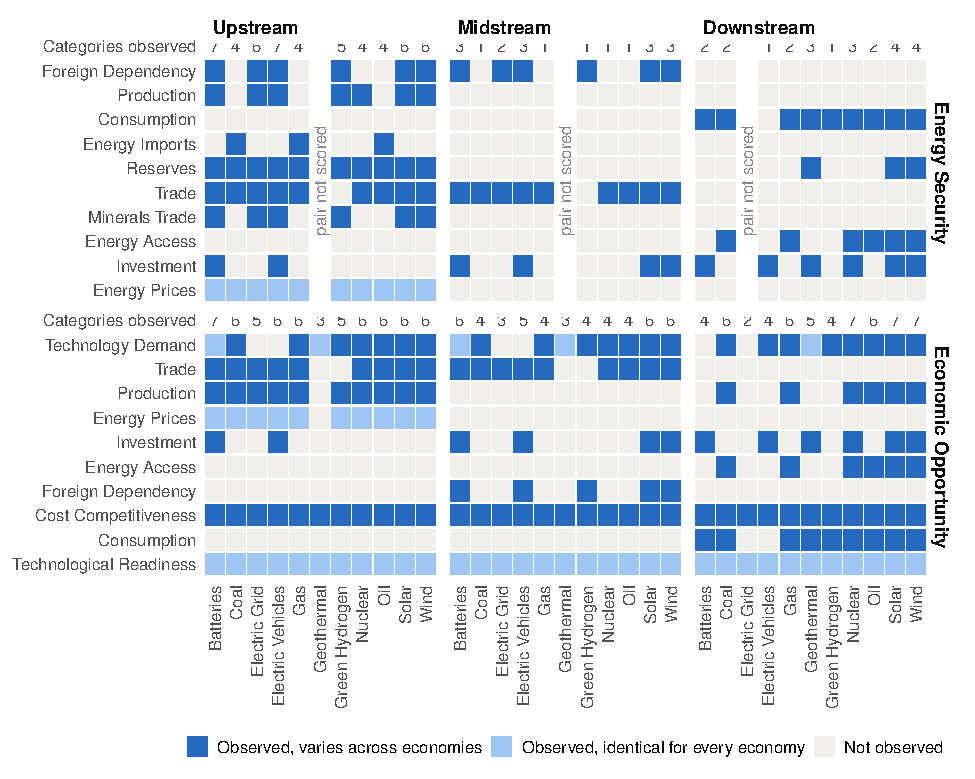
\includegraphics[width=\textwidth]{method_category_sets}
  \caption{Category composition of the pillars by technology--stage pair. Each column is one of
  the 33 headline technology--stage pairs, grouped by stage. Each row is a category of the
  Energy Security pillar (upper block) or the Economic Opportunity pillar (lower block), ordered
  by nominal weight as in Table~\ref{tab:category_weights}. Dark blue: the category is observed
  in the pair and its score varies across economies. Light blue: the category is observed but
  takes the same score for every economy of the pair (a world- or technology-level input).
  Gray: the category is not observed in the pair. The number above each column is the number
  of observed categories, which is the same for every economy of the pair. ``Pair not scored''
  marks the three pairs without an $\ES$ value. Sample: the country--technology--stage cells of
  the eleven headline technologies that have a pillar value (6,232 for $\ES$, 7,131 for $\EO$).
  Source: category contributions in \texttt{data/processed/outputs/index\_outputs.rds};
  \texttt{scripts/paper/fig\_method.R}.}
  \label{fig:method_category_sets}
\end{figure}

\paragraph{Effective weights and constant inputs.} Averaging effective weights over cells instead
of pairs changes the stage means by at most 0.032, because the category set is common within a
pair; the largest gap between effective and nominal share is 0.49. Upstream $\ES$ weight is spread
more evenly, led by Reserves (0.20), Trade (0.18) and Production (0.18); Energy Prices, nominally
0.048, carries 0.10. In $\EO$ the redistribution favours categories observed at every stage:
Technology Demand (0.20 to 0.25, nominal 0.133), Cost Competitiveness (0.19 to 0.24, nominal 0.100)
and Technological Readiness (0.12 to 0.16, nominal 0.067). Categories constant within the pair take
a mean of 0.34 of the weight of an upstream $\EO$ cell, 0.22 at the midstream stage and 0.18
downstream; adding the constant components inside varying categories (world export concentration in
Trade; the addressable-market, global-demand and overcapacity terms of Technology Demand) raises
these shares to 0.46, 0.39 and 0.27. The corresponding component-level shares in $\ES$ are 0.16,
0.20 and 0, the midstream figure being the world export-concentration term of Trade. Energy Prices
is copied to every economy before ranking, so the economies of a technology form one block of tied
ranks: with $T$ technologies the technology in position $p$ receives a percent rank close to
$(p-\tfrac12)/T$ rather than $(p-1)/(T-1)$, and no technology scores exactly 0 or 1.

\paragraph{Imputation burden by category.} Table~\ref{tab:method_imputation} gives the values
behind Figure~\ref{fig:method_imputation}. Upstream, Reserves (0.84) alone accounts for 0.17 of the
$\ES$ stage mean of 0.41; Energy Imports (0.55), Foreign Dependency (0.50) and Production (0.43)
also cover only part of the grid, and the upstream Trade category is imputed at 0.19. In $\EO$,
Technology Demand is imputed at 0.73 to 0.86 and contributes 0.16 to 0.19 to each stage mean: the
addressable-market term counts as imputed for every economy but the United States, the regional
outlook is observed for a median of 12 economies per pair, and the world-level global-demand series
is recorded for 108 economies and filled with the same value for the rest. Investment is imputed at
0.64 to 0.83 in both pillars. World-level series show almost no imputation (Energy Prices below
0.01, Technological Readiness at most 0.04), which is why $\iota_{its}$ records how a value was
obtained rather than whether it is country-specific, and why the rankability rule can admit a cell
whose observed weight is largely world-level. A component averaged across two themes counts as
imputed if either value was, so $\iota_{its}$ is an upper bound there. At the other extreme, 2,055
$\ES$ cells (33 percent) and 407 $\EO$ cells (6 percent) contain no imputed component. Rebuilding
$\iota_{its}$ from the variable table reproduces the builders' value to within $1.1\times10^{-16}$.

% Generated by scripts/paper/fig_method.R; do not edit by hand.
\begin{table}[tbp]
  \centering
  \small
  \begin{threeparttable}
    \caption{Mean imputed share by category, stage and pillar, headline technologies}\label{tab:method_imputation}
    \begin{tabular}{@{}l *{6}{S[table-format=1.2]}@{}}
      \toprule
      & \multicolumn{3}{c}{Energy Security} & \multicolumn{3}{c@{}}{Economic Opportunity}\\
      \cmidrule(lr){2-4}\cmidrule(l){5-7}
      {Category} & {Up} & {Mid} & {Down} & {Up} & {Mid} & {Down} \\
      \midrule
      Consumption & {--} & {--} & 0.03 & {--} & {--} & 0.05 \\
      Cost Competitiveness & {n.a.} & {n.a.} & {n.a.} & 0.34 & 0.42 & 0.36 \\
      Energy Access & {--} & {--} & 0.65 & {--} & {--} & 0.66 \\
      Energy Imports & 0.55 & {--} & {--} & {n.a.} & {n.a.} & {n.a.} \\
      Energy Prices & 0.01 & {--} & {--} & 0.01 & {--} & {--} \\
      Foreign Dependency & 0.50 & 0.54 & {--} & {--} & 0.79 & {--} \\
      Investment & 0.83 & 0.78 & 0.64 & 0.83 & 0.78 & 0.66 \\
      Minerals Trade & 0.02 & {--} & {--} & {n.a.} & {n.a.} & {n.a.} \\
      Production & 0.43 & {--} & {--} & 0.68 & {--} & 0.55 \\
      Reserves & 0.84 & {--} & 0.10 & {n.a.} & {n.a.} & {n.a.} \\
      Technological Readiness & {n.a.} & {n.a.} & {n.a.} & 0.04 & 0.02 & 0.03 \\
      Technology Demand & {n.a.} & {n.a.} & {n.a.} & 0.86 & 0.73 & 0.83 \\
      Trade & 0.19 & 0.01 & {--} & 0.26 & 0.15 & {--} \\
      \midrule
      Pillar, $\bar\iota$ & 0.41 & 0.23 & 0.27 & 0.41 & 0.44 & 0.43 \\
      Cells & {2,181} & {2,002} & {2,049} & {2,394} & {2,346} & {2,391} \\
      \bottomrule
    \end{tabular}
    \begin{tablenotes}[flushleft]\footnotesize
      \item \emph{Notes:} Category rows give the mean, over the country-technology-stage cells
      of the eleven headline technologies in which the category is observed, of the share of the
      category score carried by imputed components,
      $\sum_v\lambda_{vkits}\1[\tilde x_{itsv}\text{ imputed}]$. The pillar row gives the mean
      over all scored cells of the stage of the imputed weight share $\iota_{its}$ of
      equation~\eqref{eq:imputed_share}. --: category not observed at that stage; n.a.: category
      not part of the pillar. Source: \texttt{data/processed/outputs/index\_outputs.rds}
      (variable contributions and the pillar diagnostics); \texttt{scripts/paper/fig\_method.R}.
    \end{tablenotes}
  \end{threeparttable}
\end{table}


\paragraph{Mass points and pair status.} Economies without country-specific data share one value
within their pair: in five $\EO$ pairs (Electric Grid downstream, Green Hydrogen upstream and
midstream, Geothermal upstream and midstream) 65 to 70 economies sit at a single interior value,
and none of these cells is rankable. Observed zeros create mass points that the rule does not
remove: in $\ES$, 98 of the 109 economies scored in Green Hydrogen midstream share the pair's
minimum (0.256), 95 of them rankable, and in Nuclear upstream 127 of 218 share one value (0.172),
105 of them rankable. Such a tie records a real absence of production or resources but becomes a
uniform, sector-wide need under the security-need reading of the Strategic Index. A pair is
\emph{unscored} if no economy has an observed category, \emph{constant} if at least two are scored
and their range is at most $10^{-12}$, and \emph{ok} otherwise. Over every technology, including
those outside the headline set, all 45 $\ES$ pairs and all 40 $\EO$ pairs are ok; Nuclear upstream,
constant before the uranium data were added, now varies. Electric Grid downstream and Geothermal
upstream and midstream have no observed $\ES$ category.

\paragraph{Rankability in detail.} Table~\ref{tab:method_rankability} gives the counts behind
Figure~\ref{fig:method_rankability}. Counted over sovereign cells only, the rule keeps 74 percent of
$\ES$ and 67 percent of $\EO$ cells. Rankable sovereign cells score higher on average than sovereign
cells over the threshold in every pillar and stage, most markedly in midstream $\ES$ (0.46 against
0.30) and midstream $\EO$ (0.49 against 0.37). The narrowest pairs keep a usable comparison set:
Green Hydrogen midstream keeps 40 rankable $\EO$ cells (19 percent of those scored), and Nuclear
downstream, the narrowest $\ES$ pair, keeps 68. The 17 sovereign states without a rankable $\EO$
cell are Liechtenstein, Monaco, Djibouti, Dominica, Eritrea, Haiti, Kiribati, the Marshall Islands,
Micronesia, Nauru, North Korea, Palau, S\~ao Tom\'e and Pr\'incipe, Somalia, St Kitts and Nevis,
St Vincent and the Grenadines and Tuvalu; their only rankable $\EO$ cells had been upstream, and the
upstream Trade category, whose export-size and comparative-advantage terms are imputed for
economies absent from the Comtrade reporter file, lifted their imputed share just over the
threshold. Taiwan keeps 19 rankable $\ES$ and 18 rankable $\EO$ cells. In the Strategic Index the 29
policy-scored economies that lose every cell are nine territories and special administrative
regions (among them Hong Kong, Macau and the West Bank and Gaza) and 20 sovereign states: the 17
above, Andorra, the Central African Republic and Grenada. The pillars are built before the rule is
applied, so excluding a cell does not change the ranking of the cells that remain.

% Generated by scripts/paper/fig_method.R; do not edit by hand.
\begin{table}[tbp]
  \centering
  \small
  \begin{threeparttable}
    \caption{Rankable cells by pillar and stage, headline technologies}\label{tab:method_rankability}
    \begin{tabular}{@{}l *{4}{r} S[table-format=1.2] r@{}}
      \toprule
      & {Scored} & {Rankable} & \multicolumn{2}{c}{Not rankable} & {Share} & {Economies} \\
      \cmidrule(lr){4-5}
      & {cells} & {cells} & {Territory} & {$\iota_{its}>0.5$} & {rankable} & {ranked} \\
      \midrule
      \multicolumn{7}{@{}l}{\emph{Energy Security}} \\
      \quad Upstream & 2,181 & 1,124 & 231 & 826 & 0.52 & 195 \\
      \quad Midstream & 2,002 & 1,397 & 169 & 436 & 0.70 & 192 \\
      \quad Downstream & 2,049 & 1,642 & 207 & 200 & 0.80 & 193 \\
      \quad All stages & 6,232 & 4,163 & 607 & 1,462 & 0.67 & 195 \\
      \multicolumn{7}{@{}l}{\emph{Economic Opportunity}} \\
      \quad Upstream & 2,394 & 1,681 & 250 & 463 & 0.70 & 178 \\
      \quad Midstream & 2,346 & 1,307 & 221 & 818 & 0.56 & 166 \\
      \quad Downstream & 2,391 & 1,313 & 247 & 831 & 0.55 & 169 \\
      \quad All stages & 7,131 & 4,301 & 718 & 2,112 & 0.60 & 178 \\
      \bottomrule
    \end{tabular}
    \begin{tablenotes}[flushleft]\footnotesize
      \item \emph{Notes:} Country--technology--stage cells of the eleven headline technologies
      with a pillar value. A cell is rankable when the economy is a sovereign state (a Correlates
      of War state-system code) and at most $\tau=0.5$ of its index weight rests on imputed components, $\iota_{its}\le\tau$
      (\texttt{config/rankability.yml}). Reasons are exclusive: a territory is counted as a territory
      whatever its imputed share; the next column counts sovereign cells over the threshold.
      Economies ranked: economies with at least one rankable cell. Source:
      \texttt{data/processed/outputs/index\_outputs.rds}; \texttt{scripts/paper/fig\_method.R}.
    \end{tablenotes}
  \end{threeparttable}
\end{table}

